\documentclass[10pt]{article}
\usepackage{amsmath}
\usepackage{geometry}
\usepackage{fancybox}
\usepackage{tikz}
\usepackage{listings}
 \geometry{
 a4paper,
 total={170mm,257mm},
 left=20mm,
 top=-5mm,
 }

\linespread{1.3}

\title{CSC263H1 Assignment 3}
\author{Jiatao Xiang, Xu Wang, Huakun Shen}
\date{February 14th, 2019}

\begin{document}
\maketitle

\section*{Question 1}
\ovalbox{
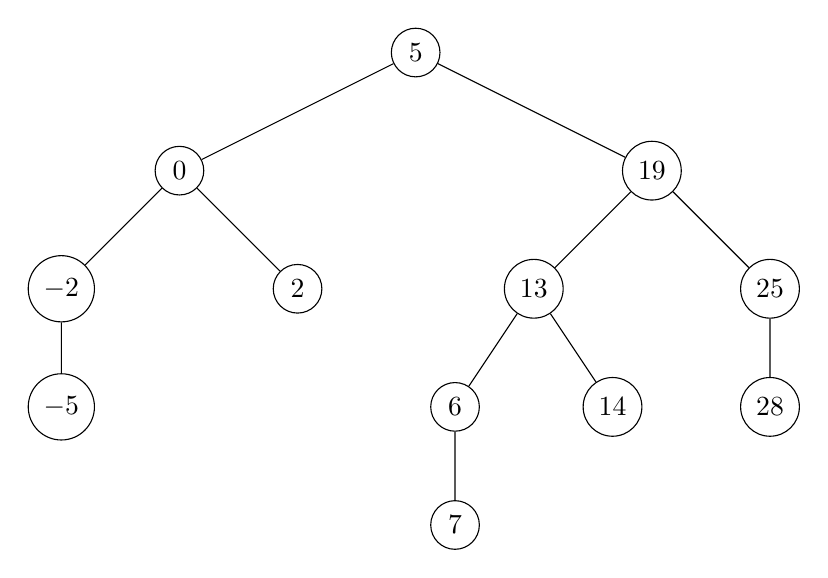
\begin{tikzpicture}[level/.style={sibling distance=60mm/#1}]
\node [circle,draw] (z){$5$}
  child {node [circle,draw] (lz) {$0$}
    child {node [circle,draw] (llz) {$-2$}
      child {node [circle, draw] (lllz) {$-5$}
      } 
    }
    child {node [circle,draw] (lrz) {$2$}
    }
  }
  child {node [circle,draw] (rz) {$19$}
    child {node [circle,draw] (rlz) {$13$}
    	child {node [circle, draw] (rllz) {$6$}
    		child {node [circle, draw] (rllrz) {$7$}}
    	}
    	child {node [circle, draw] (rlrz) {$14$}}
    }
  child {node [circle,draw] (rrz) {$25$}
    child {node [circle, draw] (rrrz) {$28$}}
	}
%\path (b) -- (g) node [midway] {+};
%\path (k) -- (l) node [midway] {+};
%\path (k) -- (g) node [midway] {+};
%\path (o) -- (p) node [midway] {+};
%  child [grow=down] {
%    node (y) {$O\left(\displaystyle\sum_{i = 0}^k 2^i %\cdot \frac{n}{2^i}\right)$}
%    edge from parent[draw=none]
%  };
%\path (q) -- (r) node [midway] {+};
%\path (s) -- (r) node [midway] {+};
%\path (s) -- (t) node [midway] {+};
%\path (s) -- (l) node [midway] {=};
%\path (t) -- (u) node [midway] {+};
%\path (z) -- (u) node [midway] {=};
%\path (j) -- (t) node [midway] {=};
%\path (y) -- (x) node [midway] {$\Downarrow$};
%\path (v) -- (y)
%  node (w) [midway] {$O\left(\displaystyle\sum_{i = 0}%^k n\right) = O(k \cdot n)$};
%\path (q) -- (v) node [midway] {=};
%\path (o) -- (x) node [midway] {+};
%\path (y) -- (w) node [midway] {$=$};
%\path (v) -- (w) node [midway] {$\Leftrightarrow$};
%\path (r) -- (c) node [midway] {$\cdots$};
};
\end{tikzpicture}
}
\section*{Question 2}


\section*{Question 3}


\end{document}
